
\documentclass[12pt]{article}

\usepackage[utf8]{inputenc}
\usepackage[greek, english]{babel}

% Packages
\usepackage{alphabeta}
\usepackage{amsmath}
\usepackage{amsthm}
\usepackage{caption}
\usepackage{color}
\usepackage{float}
\usepackage{fullpage}
\usepackage{graphicx}
\usepackage{hyperref}
\usepackage{latexsym}
\usepackage{listings}
\usepackage{pxfonts}
\usepackage{stackrel}
\usepackage{subfig}
\usepackage{tikz}
\usepackage{titlesec}
\usepackage[ruled,vlined]{algorithm2e}

% Commands
\newcommand{\N}{\mathbb{N}}
\newcommand{\R}{\mathbb{R}}
\newcommand{\abs}[1]{\left\lvert#1\right\rvert}
\newcommand{\code}[2]{\lstinputlisting[caption={#2}]{#1}}
\newcommand{\margin}{\hspace{4pt}}
\newcommand{\norm}[1]{\left\lVert#1\right\rVert}

% Environments
\newenvironment{matlab}
	{\begin{figure}[H]\centering\captionsetup{justification=centering}}
	{\end{figure}}

\newenvironment{rcases}
	{\left.\begin{aligned}}
	{\end{aligned}\right\rbrace}

% Python Syntax Highlighting
\definecolor{string_color}{RGB}{0, 161, 13}
\definecolor{comment_color}{RGB}{46, 46, 46}
\definecolor{keyword_color}{RGB}{0, 112, 191}
\definecolor{background_color}{RGB}{250, 250, 250}

\lstset{
    framesep=15pt,
    xleftmargin=15pt,
    xrightmargin=15pt,
    language=Python,
    captionpos=b,
    numbers=right,
    numberstyle=\small\ttfamily,
    frame=lines,
    showspaces=false,
    showtabs=false,
    breaklines=true,
    showstringspaces=false,
    breakatwhitespace=true,
    commentstyle=\color{comment_color}\textit,
    keywordstyle=\bfseries\color{keyword_color}\textbf,
    stringstyle=\color{string_color}\textit,
    morekeywords={self, lambda, __init__, __del__, __name__, for, in, not, and, or, :},
    basicstyle=\small\ttfamily,
    tabsize=4,
    keepspaces=true,
    columns=flexible,
    backgroundcolor=\color{background_color}
}

% Links
\hypersetup{
    colorlinks=true,
    linkcolor=blue,
    filecolor=magenta,
    urlcolor=cyan,
}

% Lengths
\setlength{\parindent}{0in}
\setlength{\oddsidemargin}{0in}
\setlength{\textwidth}{6.5in}
\setlength{\textheight}{10in}
\setlength{\topmargin}{-1.0in}
\setlength{\headheight}{18pt}

\titlespacing*{\subsection}
{0pt}{5.5ex plus 1ex minus .2ex}{4.3ex plus .2ex}

\title{\hugeΥπολογιστική Γεωμετρία\\Πρώτη Εργασία}
\author{Σιώρος Βασίλειος - 1115201500144\\Ανδρινοπούλου Χριστίνα - 1115201500006}
\date{Μάρτιος 2020}

\begin{document}

\maketitle

\pagenumbering{gobble}

\pagebreak


\subsection*{1. Implement an algorithm that takes as input three points in the plane. Checks
that they form a triangle and whether the interior of the triangle contains the origin (0, 0) or
not.}

\subsubsection*{Thought Process}

Γνωρίζουμε ότι τρία σημεία στο δισδιάστατο χώρο μπορούν είτε να σχηματίζουν ένα τρίγωνο, είτε να είναι συνευθειακά και τα τρία. \\

 Τρία σημεία καλούνται συνευθειακά στον δισδιάστατο χώρο όταν ανήκουν στην ίδια ευθεία. \\

 Η βασική ιδέα για να μπορέσουμε να εξακριβώσουμε αν τρία σημεία σχηματίζουν τρίγωνο ή όχι είναι να υπολογίσουμε το εμβαδόν του εν δυνάμει τριγώνου. Αν το εμβαδόν είναι θετικό σημαίνει ότι όντως τα τρία σημεία που έχουν επιλεχθεί σχηματίζουν τρίγωνο, ενώ αν το εμβαδόν είναι ίσο με μηδέν, τότε τα σημεία είναι συνευθειακά. \\

Το εμβαδόν του τριγώνου για τρία σημεία, έστω τα \(A(x_0, y_0)\), \(B(x_1, y_1)\), \(C(x_2, y_2)\), υπολογίζεται από τον τύπο:

\begin{align*}
E_{(ABC)} &= \frac{1}{2} \cdot
\begin{vmatrix}
1 & x_0 & y_0 \\
1 & x_1 & y_1 \\
1 & x_2 & y_2 \\
\end{vmatrix} \\
E_{(ABC)} &= \frac{1}{2} \cdot (
\begin{vmatrix}
x_1 & y_1 \\
x_2 & y_2
\end{vmatrix} -
x_0 \cdot
\begin{vmatrix}
1 & y_1 \\
1 & y_2
\end{vmatrix} +
y_0 \cdot
\begin{vmatrix}
1 & x_1 \\
1 & x_2
\end{vmatrix}) \\
E_{(ABC)} &= \frac{1}{2} \cdot (
(x_1 \cdot y_2 - x_2 \cdot y_1) - x_0(y_2 - y_1) + y_0(x_2 - x1))\\
E_{(ABC)} &= \frac{1}{2} \cdot (
x_1 \cdot y_2 - x_2 \cdot y_1 - x_0 \cdot y_2 + x_0 \cdot y_1 + y_0 \cdot x_2 - y_0 \cdot x_1)\\
E_{(ABC)} &= \frac{1}{2} \cdot (
x_0(y_1 - y_2) + x_1 (y_2 - y_0) + x_2(y_0 - y_1))\\
\end{align*}

Ουσιαστικά, το εμβαδόν του τριγώνου (ABC) είναι το μισό εμβαδόν του παραλληλογράμμου που ορίζεται από δύο διανύσματα που εχουν κοινή κορυφή είτε το A, είτε το B, είτε το C, ανάλογα με την επιλογή που θα κάνουμε. Το εμβαδόν αυτή της περιοχής είναι το εξωτερικό γινόμενο των δύο διανυσμάτων.\\

Με αυτόν τον τρόπο αποφεύγεται ο υπολογισμός του ύψους του τριγώνου που απαιτείται από τον κλασσικό τύπο υπολογισμού εμβαδού τριγώνου:

\begin{align*}
E_{triangle} = \frac{base\cdot height}{2}
\end{align*}

Αν έχουμε καταλήξει πως τα δοθέντα σημεία σχηματίζουν ένα τρίγωνο, τότε πρέπει να ελεχθεί αν το σημείο Ο(0,0) ανήκει μέσα στο τρίγωνο. Υπολογίζονται τα εμβαδά των τριγώνων ABO, AOC και OBC, με τον τρόπο που αναφέρθηκε παραπάνω. Αν το αθροισμά των εμβαδών αυτών είναι ίσο με το εμβαδόν του τριγώνου ABC,

\begin{align*}
E_{(AB0)} + E_{(A0C)} + E_{(0BC)} = E_{(ABC)}
\end{align*}

τότε το O βρίσκεται στο εσωτερικό του τριγώνου, διαφορετικά βρίσκεται εκτός του τριγώνου. \\

Αν για λίγο μεταβούμε στον τρισδιάστατο χώρο και θεωρήσουμε ότι το τρίγωνο ABC βρίσκεται στο επίπεδο E και το σημείο που επιθυμούμε να ελέγξουμε βρίσκεται στο χώρο εκτός του επιπέδου Ε, σχηματίζοντας τα τρία τρίγωνα που αναφέρονται παραπάνω, προκύπτει μία πυραμίδα με τριγωνική βάση. Επιλέγουμε να κανονικοποιήσουμε τις ακμές, για να μην προκύψουν λανθασμένα αποτελέσματα. Η μοναδική περίπτωση που το άθροισμα των εμβαδών των τριών εδρών που προύπτουν από το υπό εξέταση σημείο και δύο άλλα σημεία του αρχικού τριγώνου να ισούται με το εμβαδόν του αρχικού τριγώνου είναι το σημείο να βρίσκεται σε τέτοια θέση, ώστε η προβολή του στο επίπεδο E να συμπίπτει με κάποιο από τα εσωτερικά σημεία του τριγώνου ή με τις κουρυφές αυτού. \\

\subsubsection*{Implementation}

Παραθέτουμε τον αλγόριθμο που υλοποιεί όσα αναφέρθηκαν παραπάνω. Η υλοποίηση αυτού έγινε σε γλώσσα python και εντοπίζεται στο αρχείο exercise1.py του παραδοταίου αρχείου.

\begin{algorithm}[H]
	\SetAlgoLined
	\KwResult{Τα σημεία δημιουργούν/ δε δημιουργούν τρίγωνο. Το σημείο O(0,0) ανήκει / δεν ανήκει στο τρίγωνο}

	A, B, C = Δώσε είσοδο 3 σημεία \;
	Έλεγχος αν τα σημεία δημιουργούν τρίγωνο \;
	\eIf{δημιουργείται τρίγωνο}
	{Τύπωσε κατάλληλο μήνυμα \;
	Έλεγχος αν το σημείο (0,0) βρίσκεται εντός του τριγώνου \;}
	{Τύπωσε κατάλληλο μήνυμα \;}

	\caption{Έλεγχος σχηματισμού τριγώνου και εντοπισμός του σημείου O(0,0) εντός ή εκτός τριγώνου}
\end{algorithm}

\begin{algorithm}[H]
	\SetAlgoLined
	\KwResult{True / False}

	\(Ε\) = Υπολογισμός του εμβαδού του σχήματος που σχηματίζεται από τα A, B, C \;
	\eIf{\( Ε > 0\)}
	{Επέστρεψε True \;}
	{Επέστρεψε False \;}

	\caption{Έλεγχος αν τα σημεία δημιουργούν τρίγωνο}
\end{algorithm}

\begin{algorithm}[H]
	\SetAlgoLined
	\KwResult{Το σημείο O(0,0) ανήκει / δεν ανήκει στο τρίγωνο}

	\(E\) = Υπολογισμός του εμβαδού του σχήματος που σχηματίζεται από τα A, B, C \;
	\(E_1\) = Υπολογισμός του εμβαδού του σχήματος που σχηματίζεται από τα A, B, O \;
	\(E_2\) = Υπολογισμός του εμβαδού του σχήματος που σχηματίζεται από τα A, O, C \;
	\(E_3\) = Υπολογισμός του εμβαδού του σχήματος που σχηματίζεται από τα O, B, C \;
	\eIf{\(E_1 + E_2 + E_3 = E\)}
	{Τύπωσε "Το σημείο O(0,0) ανήκει" \;}
	{Τύπωσε "Το σημείο O(0,0) δεν ανήκει" \;}

	\caption{Έλεγχος αν το σημείο (0,0) βρίσκεται εντός του τριγώνου}
\end{algorithm}

\subsubsection*{Implementation}

Στο αρχείο exercise1.py βρίσκεται ο κώδικας που υλοποιεί όσα αναφέρθηκαν στις παραγράφους Thought Process και Algorithms. Η υλοποίηση βασίζεται στον υπολογισμό εμβαδών τριγώνων. Πιο συγκεκριμένα, χρησιμοποιείεται η συνάρτηση του Figure 1. \\

\begin{matlab}
	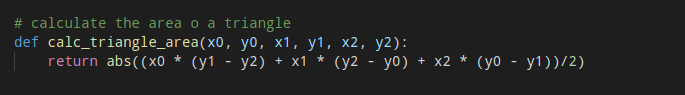
\includegraphics[scale=0.6]{images/exercise1_impl.png}
  	\caption{Συνάρτηση υπολογισμού εμβαδού τριγώνου}
\end{matlab}

Έγινε χρήση της abs(), για να αποφύγουμε αρνητικές τιμές. Με αυτόν τον τρόπο προκύπτουν μόνο θετικές τιμές ή το μηδέν. Για τους σκοπούς του πρώτου ερωτήματος θα μπορούσαμε να αποφύγουμε τη διαίρεση με το 2, για να αποφευχθεί μία επιπλέον πράξη που δεν επηρεάζει σημαντικά το αποτέλεσμα, καθώς στο πρώτο ερώτημα δε μας ενδιαφέρει το ακριβές αποτέλεσμα, αλλά αν το εμβαδόν "υπάρχει" ή όχι, δηλαδή αν είναι θετικό ή αρνητικό. Ωστόσο, είναι απαραίτητο να υπολογιστεί ακριβώς η τιμή του εμβαδού για τα τρίγωνα του δεύτερου ερωτήματος, οπότε επιλέξαμε να κρατήσουμε καθολικά την ίδια συνάρτηση για όλη την υλοποίηση, καθώς δεν αποτελεί σημαντική βελτιστοποίηση στην παρούσα φάση. \\

Έπειτα το πρόγραμμα ελέγχει αν τα τρία αυτά σημεία σχηματίζουν ένα τρίγωνο ή όχι. Ο έλεγχος γίνεται υπολογίζοντας το εμβαδόν της περιοχής που σχηματίζεται από τα τρία σημεία του input. Αν το εμβαδόν είναι 0 σημαίνει ότι τα σημεία που δόθηκαν είναι συνευθειακά και συνεπώς δεν σχηματίζουν τρίγωνο, ενώ σε οποιαδήποτε άλλη περίπτωση, τα σημεία θα ορίζουν ένα τρίγωνο. \\

\subsubsection*{Running the code}

Το πρόγραμμα τρέχει με την εντολή ./python exercise1.py \\

Ζητά από τον χρήστη να δώσει τις ακέραιες συντεταγμένες 3 σημειών στον χώρο. Οι συντεταγμένες που δίνονται από τον χρήστη για κάθε σημείο πρέπει να διαχωρίζονται με κενό. Υπάρχουν παραδείγματα εισόδου στα Figures 3 και 5. \\

Έπειτα, το πρόγραμμα παράγει τα αποτελέσματα και τις αντίστοιχες γραφικές παραστάσεις. \\

Πιο συγκεκριμένα, απαντά "These points form a triangle" αν τα 3 σημεία που δόθηκαν από τον χρήστη σχηματίζουν τρίγωνο και "These points don't form a triangle" στην αντίθετη περίπτωση. Αν τα σημεία σχηματίζουν τρίγωνο και στο τρίγωνο αυτό περιέχεται το σημείο (0,0), τότε το πρόγραμμα απαντά "The interior of the triangle contains the origin (0, 0)". Επίσης, παράγεται η γραφική αναπαράσταση του τριγώνου αν υπάρχει, ενώ αν δεν υπάρχει τότε εμφανίζονται απλά τα σημεία τα οποία είναι συνευθειακά. Παραθέτουμε αντίστοιχα παραδείγματα εκτέλεσης του κώδικα στις εικόνες. \\

\subsubsection*{Example Usage}

\begin{matlab}
	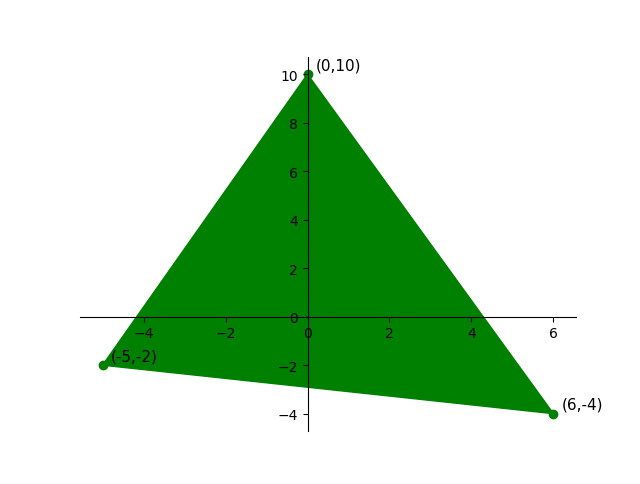
\includegraphics[scale=0.8]{images/exercise1_1.png}
	\caption{Αποτελέσματα προγράμματος με input αυτό που δίνεται στο Figure 2}
\end{matlab}

\begin{matlab}
	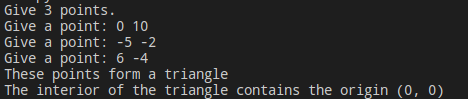
\includegraphics[scale=0.7]{images/exercise1_2.png}
	\caption{Παράδειγμα input - output προγράμματος}
\end{matlab}

\begin{matlab}
	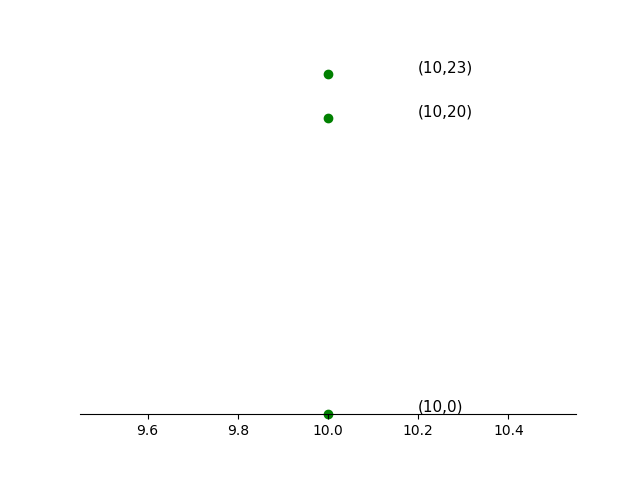
\includegraphics[scale=0.8]{images/exercise1_3.png}
	\caption{Αποτελέσματα προγράμματος με input αυτό που δίνεται στο Figure 2}
\end{matlab}

\begin{matlab}
	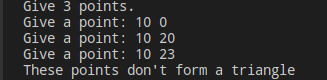
\includegraphics[scale=0.7]{images/exercise1_4.png}
	\caption{Παράδειγμα input - output προγράμματος}
\end{matlab}

\pagebreak

\subsection*{2. Given a circle of radius r in the plane with (0, 0) as center, implement an
algorithm that finds the total lattice points on the circumference. Lattice Points are points
with integer coordinates.}

\subsubsection*{Thought Process}

Σε ένα καρτεσιανό σύστημα συντεταγμένων, ένας κύκλος με κέντρο το σημείο (a, b)
και ακτίνα r είναι ένα σχήμα το οποίο αποτελείται από όλα τα σημεία των οποίων
οι συντεταγμένες ικανοποιούν την εξίσωση \\

\[ (x - a) ^ 2 + (y - b) ^ 2 = r ^ 2 \]

Από την παρπάνω εξίσωση, μπορούμε να συμπεράνουμε,
ότι οποιοδήποτε σημείο, του οποίου η Ευκλείδια απόσταση από το κέντρο του κύκλου
είναι μεγαλύτερη της ακτίνας του, βρίσκεται εκτός του κύκλου. \\

Αν ο κύκλος έχει ως κέντρο την αρχή των αξόνων, δηλαδή το σημείο \( (0, 0) \), τότε
η παραπάνω εξίσωση παίρνει την εξής απλούστερη μορφή \\

\[ x ^ 2 + y ^ 2 = r ^ 2 \]

Σε αυτή την περίπτωση, είτε η τετμημένη είτε η τεταγμένη ενός σημείου
αρκεί να είναι μεγαλύτερη της ακτίνας του έτσι ώστε να μην ανήκει στον κύκλο. \\

Ως εκ τούτου, τα σημεία πλέγματος ενός κύκλου ακτίνας r με κέντρο το (0, 0)
είναι υποσύνολο του συνόλου που απαρτίζεται από σημεία με ακέραιες συνταγμένες
στο εύρος \( [-r, +r] \) και στις δύο διαστάσεις, με την πρόσθετη συνθήκη
να ικανοποιούν την παραπάνω εξίσωση έτσι ώστε να βρίσκονται επί της
περιφέρειάς του. \\

Για παράδειγμα, για έναν κύκλο ακτίνας 1 με κέντρο το (0, 0) αρκεί να
ελέγξουμε ποιά από τα σημεία εντός του συνόλου \\

\[ \{ (-1, 0), (0, -1), (0, +1), (+1, 0) \} \]

ικανοποιούν την εξίσωση

\[ x^2 + y^2 = 1 \]

\pagebreak

\subsubsection*{Implementation}

Δεδομένου ότι δεν ήταν ξεκάθαρο, αν το πρόβλημα ζητούσε μόνο
το πλήθος ή και τα ακριβή σημεία πλέγματος,
αποφασίσαμε να ακολουθήσαμε την παρακάτω προσέγγιση η οποία μπορεί να
χρησιμοποιηθεί για την εύρεση και των δύο όπως θα δείτε
στην συνέχεια. \\

\begin{lstlisting}
def lattice_points(radius):
    points = []

    for x in range(-radius, radius + 1):
        for y in range(-radius, radius + 1):
            if x ** 2 + y ** 2 == radius ** 2:
                points.append((x, y))

    return points
\end{lstlisting}

\pagebreak

\subsubsection*{Running the code}

\begin{matlab}
    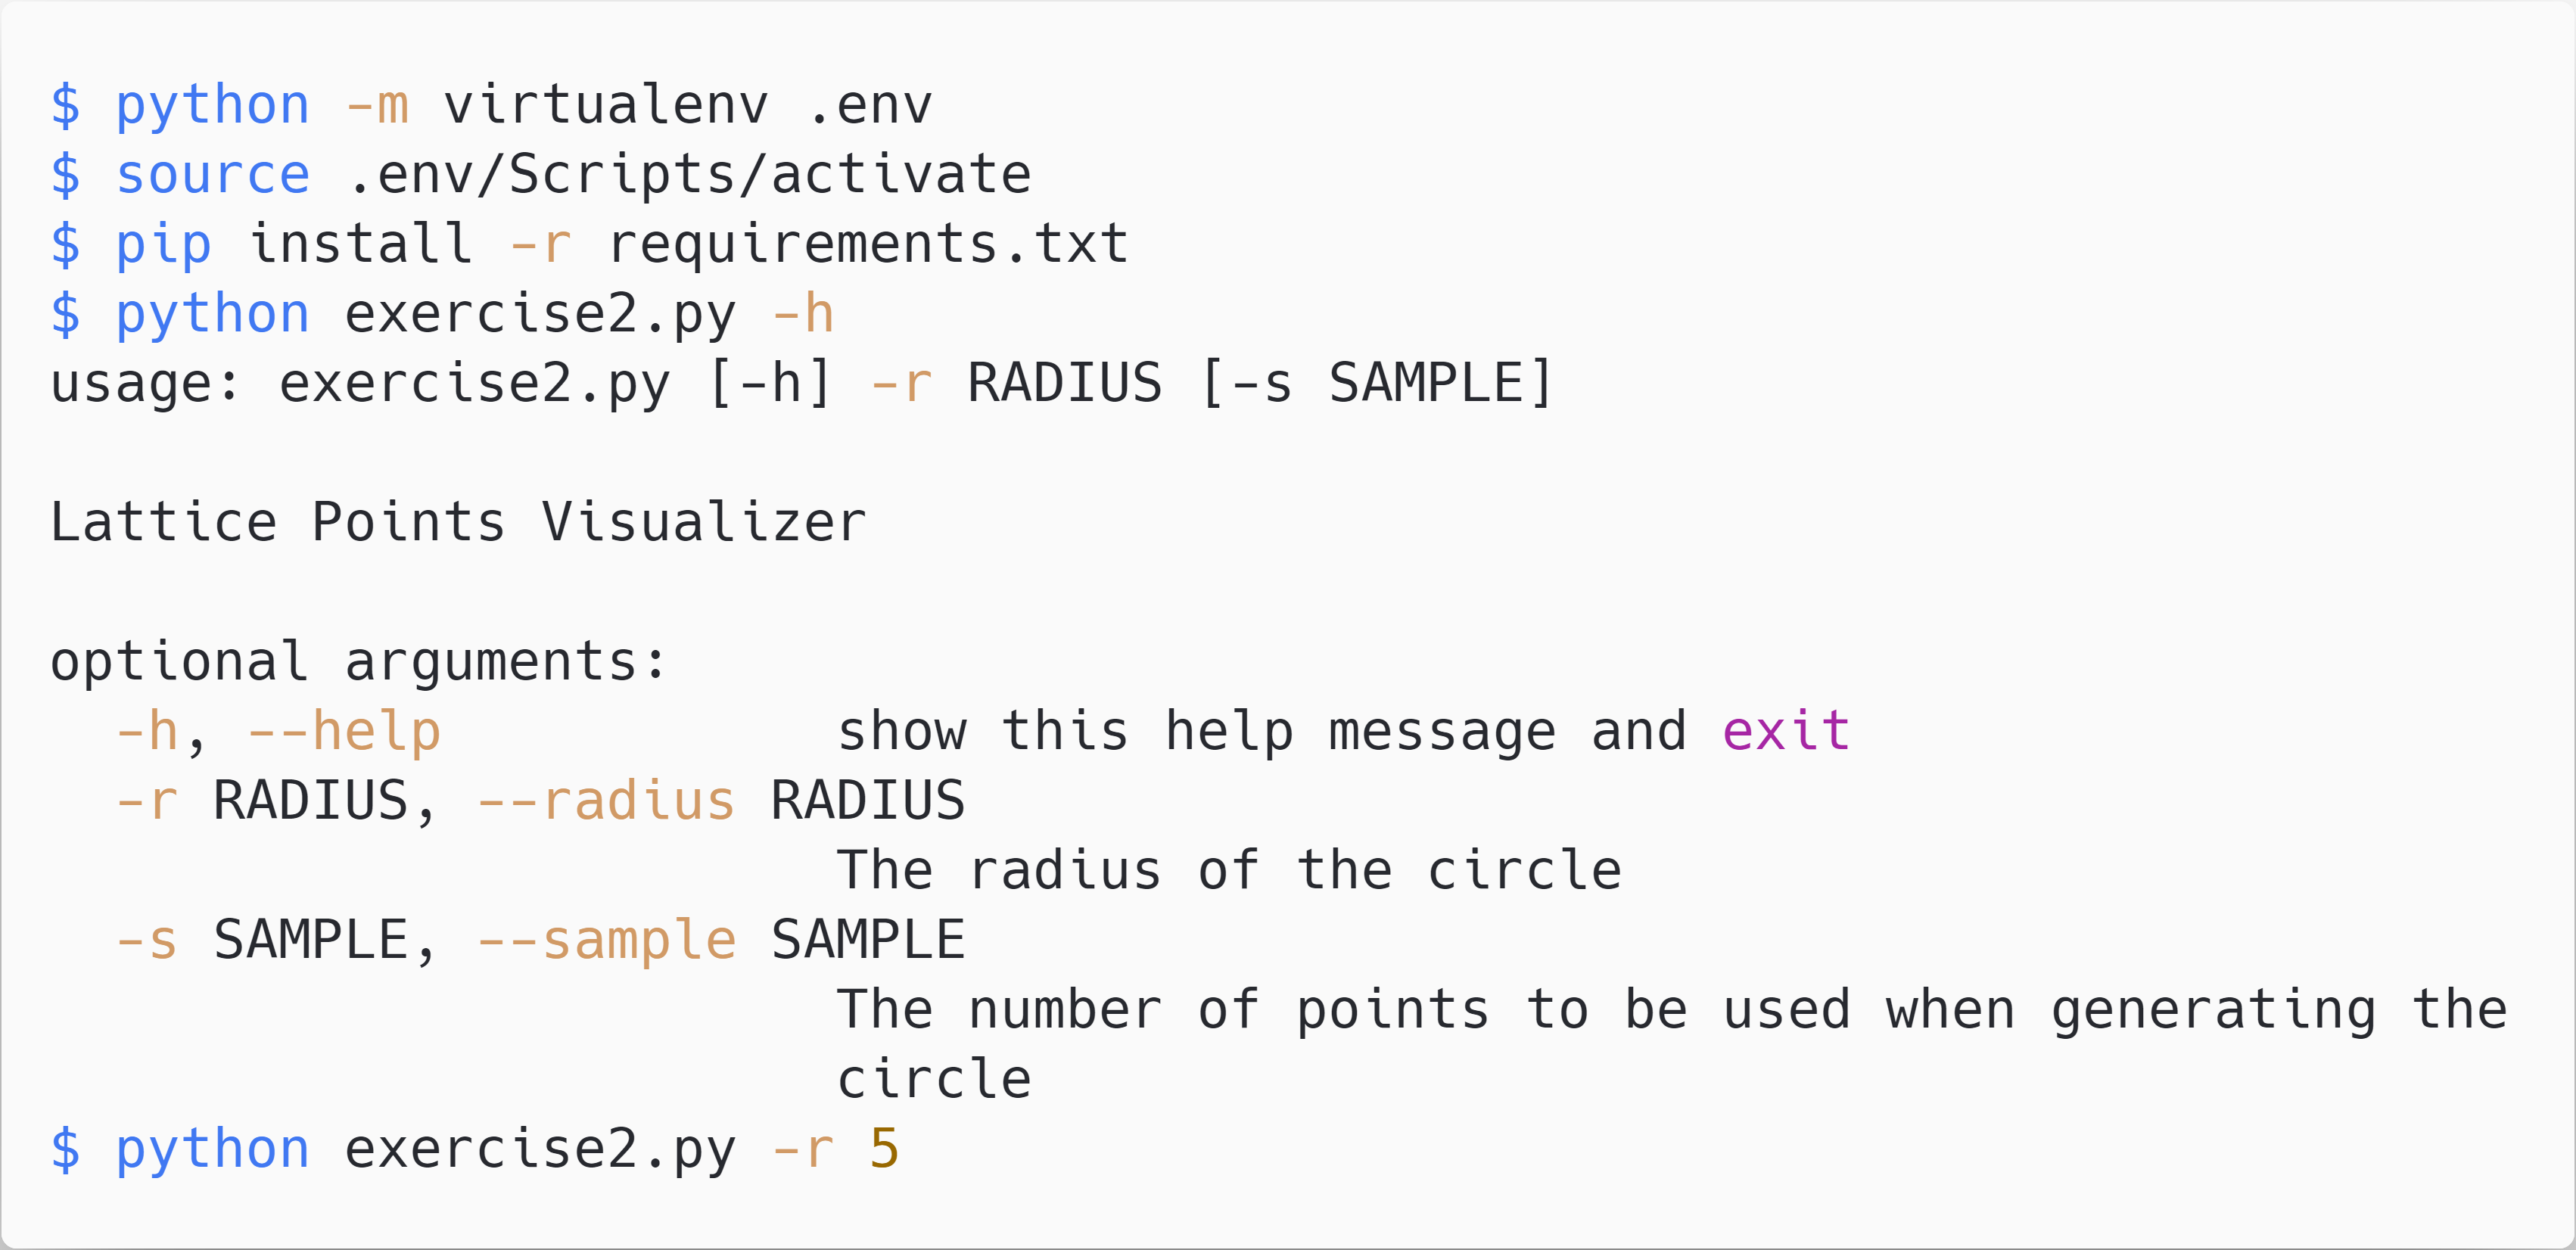
\includegraphics[scale=0.140]{images/lattice_points.png}
    \caption{Οδηγίες εκτέλεσης προγράμματος}
\end{matlab}

\subsubsection*{Example Usage}

\begin{matlab}
    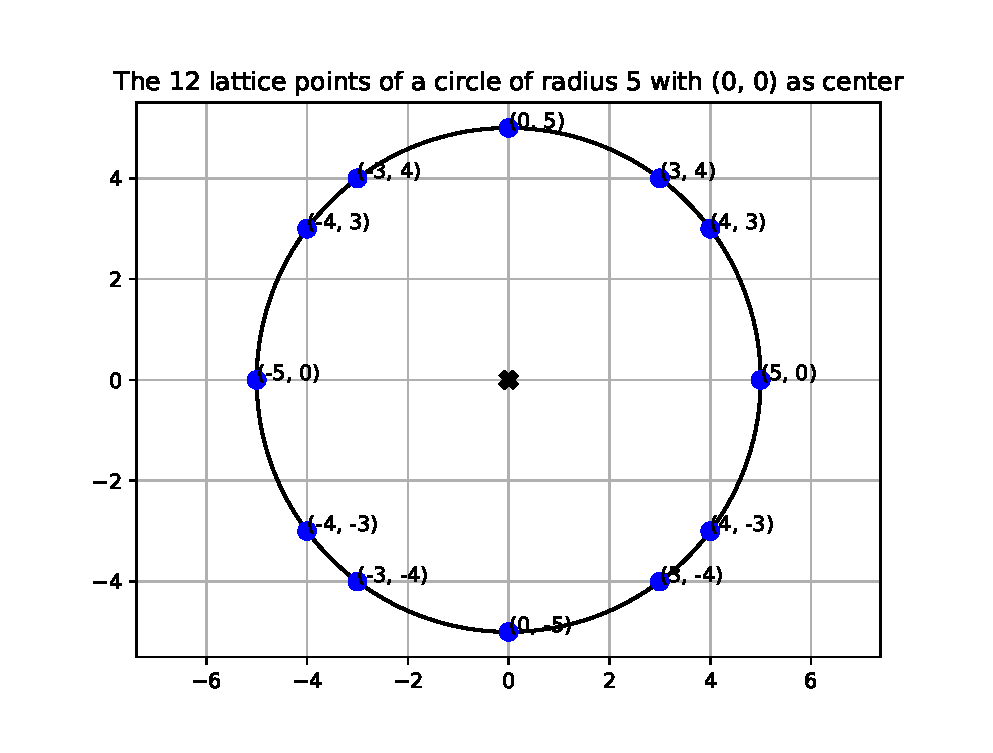
\includegraphics[scale=1]{images/lattice_points.eps}
    \caption{Ενδεικτική έξοδος του προγράμματος}
\end{matlab}

\pagebreak

\subsection*{3. Implement the incremental 2D algorithm for computing the convex hull of a
finite set of points in the plane.}

\subsubsection*{Thought Process}

Στόχος τους αυξητικού αλγορίθμου ή αλλιώς beneath-beyond αλγορίθμου είναι να δημιουργήσει ένα κατάλληλο κυρτό περίβλημα βασιζόμενος σε ένα σύνολο σημείων στον δισδιάστατο χώρο (επεκτείνεται και σε περισσότερες διαστάσεις), το οποίο να περιλαμβάνει όλα τα σημεία που του δόθηκαν ως είσοδος. Ο αυξητικός αλγόριθμος καλείται έτσι διότι εξετάζει σημεία του χώρου το ένα μετά το άλλο και κάθε φορά προσθέτει ένα σημείο στο υπό κατασκευή κυρτό περίβλημα. \\

Στην υλοποίησή μας χρησιμοποιήσαμε τον κλασσικό αλγόριθμο beneatrh beyond, ο οποίος συνοψίζεται στην επόμενη υποενότητα. \\

Αρχικά, ταξινομούμε σε φθίνουσα σειρά όλα τα σημεία του δισδιάστατου χώρου που λάβαμε ως είσοδο με πρωτεύον κριτήριο την τετμημένη τους. Έτσι, ο αλγόριθμος ξεκινά με τα σημεία που βρίσκονται δεξιά και καταλήγει σε εκείνα που βρίσκονται αριστερά, δηλαδή σαρώνει τα σημεία από δεξιά προς αριστερά. Με αυτόν τον τρόπο κάθε καινούριο σημείο που εξετάζεται από τον αλγόριθμο είναι εξωτερικό του πολυγώνου που ήδη έχει κατασκευαστεί. Επίσης το ευθύγραμμο τμήμα που σχηματίζεται από το υπό εξέταση σημείο και από το ακριβώς προηγούμενο υπό εξέταση σημείο είναι εξωτερικό του κυρτού περιβλήματος. \\

Ξεκινώντας από τα τρία δεξιότερα σημεία δημιουργούμε ένα τρίγωνο, το οποίο θεωρείται κυρτό περίβλημα στην περίπτωση που είχαμε μόνο αυτά τα τρία σημεία ως είσοδο. Ο αλγόριθμος βασίζεται στο τρίγωνο αυτό και το επεκτείνει στην κυρτή θήκη που στοχεύει να κατασκευάσει. \\

Βασικό χαρακτηριστικό του beneath-beyond είναι ο χρωματισμός των ακμών και των κορυφών. Πιο συγκεκριμένα, οι κορυφές μπορούν να λάβουν τρία διαφορετικά χρώματα και οι ακμές δύο. Μία ακμή χρωματίζεται κόκκινη στην περίπτωση που είναι ορατή από το υπό εξέταση κάθε φορά σημείο, ενώ αν δεν είναι ορατή χρωματίζεται με μπλέ χρώμα. Οι κορυφές μπορούν να λάβουν τα χρώματα: κόκκινο, μπλέ και μωβ. Μία κορυφή είναι κόκκινη όταν εντοπίζεται ανάμεσα σε δύο κόκκινες ακμές, μπλέ όταν εντοπίζεται ανάμεσα σε δύο μπλέ ακμές και μώβ όταν εντοπίζεται ανάμεσα σε μία κόκκινη και μία μπλέ ακμή. \\

Η ορατότητα κάθε ακμής από ένα σημείο υπολογίζεται με βάση το κατηγόρημα προσανατολισμού ή αλλιώς το κατηγόρημα CCW (Counter ClockWise). Κατηγόρημα ονομάζεται ο έλεγχος μίας ιδιότητας ως προς συγκεκριμένα γεωμετρικά δεδομένα. Ο έλεγχος αυτός μπορεί να παράξει δύο διακριτές τιμές (π.χ.: True/False) και σε ορισμένες περιπτώσεις μπορεί να αποδόσει και μία τρίτη τιμή, η οποία θα αφορά μία εκφυλισμένη περίπτωση. Στην περίπτωση του κατηγορήματος CCW, η είσοδός του είναι τρία σημεία και η έξοδός του είναι ο προσανατολισμός αυτών των τριών σημειών, δηλαδή η φορά της στροφής των σημείων αυτών. Αν τα τρία σημεία που δίνονται στο CCW είναι τα \(x,y,z\), το κατηγόρημα αποφασίζει αν τα διανύσματα \(\vec{v_1} = (x,y)\) και \(\vec{v_2} = (x,z)\) σύμφωνα με τον κανόνα του δεξιού χεριού ορίζουν μία θετική ή μία αρνητική στροφή. Θετική καλείται η στροφή στην οποία το εξωτερικό γινόμενο των διανυσμάτων έχει θετικό πρόσημο, ενώ σε διαφορετική περίπτωση καλείται αρνητική. Η αρνητική στροφή καλείται CW (σύμφωνη με τη φορά των δεικτών του ρολογιού) και η θετική CCW (αντίθετη με τη φορά των δεικτών του ρολογιού). Να σημειώσουμε ότι η επιλογή εδώ των διανυσμάτων έγινε με τυχαίο τρόπο και το βασικό είναι να επιλέγονται διανύσματα με κοινή κορυφή. \\

Στον αλγόριθμο η ορατότητα της ακμής καθορίζεται από τον υπολογισμό των \(CCW(a_i, a_j, a)\) και \(CCW(a_i, a_j, p)\), όπου p είναι το υπό εξεταση σημείο, τα \(a_i\) και \(a_j\) ορίζουν μία ακμή του πολυγώνου και a είναι μία οποιαδήποτε άλλη κορυφή που ανήκει στο πολύγωνο και δεν είναι μία από τις τρείς κορυφές που αναφέρθηκαν παραπάνω. \\

Αφού χρωματιστούν όλες οι ακμές και οι κορυφές κατάλληλα, ελέγχονται οι ακμές που δημιουργήθηκαν στην προηγούμενη επανάληψη και περιέχουν το προηγούμενο υπό εξέταση σημείο. Αφού έχουμε ταξινομήσει τις κορυφές ως προς τη τετμημένη το τρέχον υπό εξέταση σημείο "βλέπει" το αμέσως προηγούμενο υπό εξέταση σημείο και τουλάχιστον μία από τις ακμές που προσπίπτουν σε αυτό και κατασκευάστηκαν στο προηγούμενο βήμα. Ο αλγόριθμος εντοπίζει μία κόκκινη ακμή, με εφαλτήριο την προηγούμενη υπο εξέταση κορυφή, και ανατρέχει όλες τις ακμές, για να εντοπίσει όλες τις κόκκινες ακμές. Σταματά την αναζήτηση όταν φτάσει σε μώβ κορυφές, οι οποίες είναι συνολικά δύο σε κάθε βήμα, διότι η μισή κυρτή θήκη είναι μπλέ (από την πλευρά που δεν είναι ορατή για το σημείο που εξετάζεται) και η άλλη μισή κυρτή θήκη είναι κόκκινη (από την πλευρά που είναι ορατή από το σημείο εξέτασης). Ο αλγόριθμος διαγράφει τις κόκκινες ακμές και ενώνει το υπό εξέταση σημείο με τις δύο μωβ κορυφές. \\

Μόλις σαρώσει όλα τα σημεία που του δόθηκαν ως είσοδο, ο αλγόριθμος έχει παράξει την κυρτή θήκη που τα περιέχει όλα. \\

\subsubsection*{Implementation}

Ο αυξητικός αλγόριθμος συνοψίζεται στον αλγόριθμο 4. Η υλοποίηση αυτού έγινε σε γλώσσα python και εντοπίζεται στο αρχείο exercise3.py του παραδοταίου αρχείου.

\begin{algorithm}[H]
	\SetAlgoLined
	\KwResult{Κυρτή θήκη σημείων που δόθηκαν ως είσοδος}

	Δώσε είσοδο n σημεία \;

	Ταξινόμηση σημείων κατά φθίνουσα τετμημένη \;

	Έλεγχος αν τα τρία δεξιότερα σημεία δημιουργούν τρίγωνο \;
	\eIf{δεν δημιουργείται τρίγωνο}
	{Επέλεξε τα σημεία \((x, \min(y))\) και \((x, \max(y))\) και αγνόησε τα ενδιάμεσα\;}

	Δημιούργησε τρίγωνο Τ \;
	Αρχικοποίησε το τρέχον πολύγωνο με το τρίγωνο Τ \;

	\For{σημείο \(p_k\), όπου \(k=3,4,...,n\)}
	{Βρες όλες τις κόκκινες ακμές ξεκινόντας από τις ακμές του \(p_{k-1}\) \;
	Βρές δύο μωβ κορυφές \;
	Διέγραψε όλες τις κόκκινες ακμές \;
	Δημιούργησε δύο ακμές από το σημείο \(p_k\) στα δύο μωβ σημεία \;
	}

	\caption{Αυξητικός αλγόριθμος (beneath-beyond)}
\end{algorithm}

\subsubsection*{Implementation}

Ο αλγόριθμος beneath-beyond έχει υλοποιηθεί στο αρχείο exercise3.py του παραδοταίου. Ακολουθήθηκαν πιστά τα βήματα του αλγορίθμου. \\

Για τον έλεχγο δημιουργίας τριγώνου από τα τρία πρώτα σημεία χρησιμοποιήθηκε η αντίστοιχη συνάρτηση που ορίστηκε στο αρχείο exercise1.py, που ελέγχει το εμβαδό του πολυγώνου που δημιουργούν τα τρία σημεία. Στην περίπτωση που τα τρία δεξιότερα σημεία είναι συνευθειακά και δε μπορούν να κατασκευάσουν ένα τρίγωνο, επιλέξαμε να αγνοήσουμε τα ενδιάμεσα σημεία και να χρησιμοποιήσουμε τα σημεία \((x, \min(y))\), \((x, \max(y))\) και το επόμενο στην ταξινόμηση σημείο \((x_{next}, y')\). \\

Διατηρούμε δύο δομές για την αποθήκευση των απαραίτητων δεδομένων για τον αλγόριθμο. Η μία δομή περιέχει τις ακμές του τρέχοντος κυρτού περιβλήματος και τον αντίστοιχο χρωματισμό τους και η άλλη δομή περιέχει τις κορυφές και τον αντίστοιχο χρωματισμό αυτών. \\

Σε κάθε βήμα του αλγορίθμου, ελέγχουμε τον χρωματισμό των ακμών και τον τροποποιούμε αναλόγως με τη θέση του υπό εξέταση σημείου και έπειτα ενεργούμε αναλόγως και με τις κορυφές. Απομακρύναμε τις κόκκινες ακμές, διαγράφοντάς τες από τη δομή που αποθηκεύονται οι ακμές, διότι δε θα συνέβαλλαν στη συνέχεια του αλγορίθμου. Δημιουργούμε δύο καινούριες ακμές από το τρέχον σημείο προς τις μως κορυφές, προσθέτοντας τα αντίστοιχα δεδομένα στη δομή των ακμών και συνεχίζουμε τη διαδικασία αυτή μέχρι να παραχθεί η τελική κυρτή θήκη, δηλαδή μέχρι να εξεταστούν όλα τα σημεία της εισόδου. \\

\subsubsection*{Running the code}

Το πρόγραμμα τρέχει με την εντολή ./python exercise3.py και έχουμε δώσει τη δυνατότητα για δύο εναλλακτικούς τρόπους εισαγωγής δεδομένων. Η πρώτη επιλογή είναι με εισαγωγή των ακέραιων συντεταγμένων των σημειών από τον χρήστη. Αρχικά, ο χρήστης πρέπει να δηλώσει πόσα σημεία επιθυμεί να εξετάσει το πρόγραμμα και έπειτα να δώσει ένα προς ένα τα σημεία. Η τετμημένη και η τεταγμένη του κάθε σημείου πρέπει να διαχωρίζονται με κενό. Η δεύτερη επιλογή είναι να παράγει το ίδιο το πρόγραμμα τυχαία σημεία στον δισδιάστατο χώρο, ανάλογα με τις αντίστοιχες παραμέτρους που έχουν δοθεί στο κώδικα. Εμέις έχουμε αφήσει ενδεικτικά ένα συνδυασμό τέτοιων παραμέτρων. Με κατάλληλο σχολιασμό - αποσχολιασμό δουλεύουν και οι δύο εναλλακτικές. \\

Η έξοδος τους προγράμματος είναι ένα διάγραμμα που απεικονίζει όλα τα σημεία που δόθηκαν στην είσοδο και το αντίστοιχο κυρτό περίβλημα. Ένα τετοιο παράδειγμα φαίνεται παρακάτω. Αποφασίσαμε να οπτικοποιήσουμε την έξοδο, διότι αν η έξοδος ήταν απλά μία αλυσίδα κορυφών και ακμών που κατασκευάζουν το κυρτό περίβλημα θα ήταν δύσκολο στον χρήστη να αποφανθεί για την ορθότητα του προγράμματος. \\

\subsubsection*{Example Usage}

\begin{matlab}
	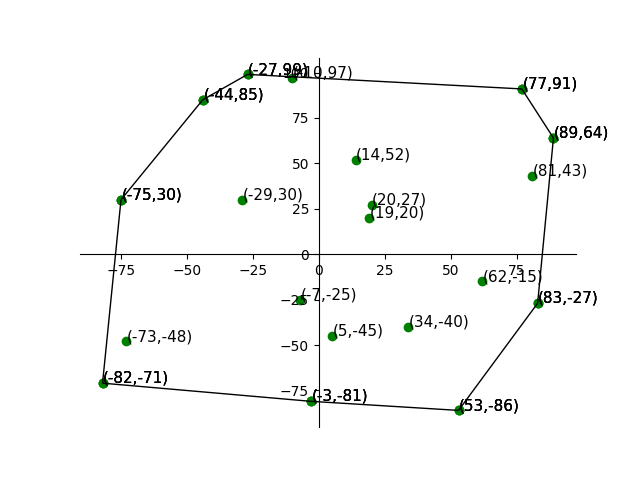
\includegraphics[scale=0.7]{images/exercise3_1.png}
	\caption{Ενδεικτική έξοδος του προγράμματος}
\end{matlab}

\pagebreak

\subsection*{4. Implement the gift wrap algorithm for computing the convex hull of a finite
set of points in the plane .}

\subsubsection*{Thought Process}

Ο \textbf{Gift Wrapping} αλγόριθμος, που στην περίπτωση των δύο διαστάσεων είναι
επίσης γνωστός και ως ο \textbf{Jarvis March} αλγόριθμος, μπορεί να περιγραφεί από τα εξής
απλά βήματα \\

\begin{enumerate}
    \item Δεδομένου ενός συνόλου σημείων στον \( \R^2 \),
    επιλέγει ένα σημείο το οποίο είναι γνωστό ότι
    ανήκει στο \textbf{Convex Hull} του συνόλου,
    όπως π.χ. το αριστερότερο σημείο μεταξύ των δεδομένων σημείων.

    \item Στη συνέχεια, επιλέγει ως επόμενο σημείο το σημείο για το οποίο,
    όλα τα υπόλοιπα σημεία βρίσκονται δεξιά της ευθείας που ορίζουν
    το τρέχον και το σημείο αυτό.

    \item Αν το τρέχον σημείο ταυτίζεται με το αρχικά επιλεχθέν σημείο,
    τότε τερμάτησε καθώς το \textbf{Convex Hull} υπολογίστηκε και αποτελείται
    από το σύνολο επιλεχθέντων σημείων έως τώρα. Διαφορετικά επανάλαβε
    το βήμα 2.
\end{enumerate}

Ο αλγόριθμος ουσιαστικά επιλέγει κάθε επόμενο σημείο έτσι ώστε
να προκύπτει η μεγαλύτερη δυνατή εσωτερική γωνία. \\

\pagebreak

\subsubsection*{Implementation}

Ορίσαμε 3 βοηθητικές συναρτήσεις

\begin{itemize}
    \item \textbf{orientation}: Υπολογίζει τον προσανατολισμο
    των δύο διανυσμάτων που ορίζουν τα 3 σημεία στην είσοδό της

    \item \textbf{counterclockwise}: Με τη βοήθεια της συνάρτηση
    \textbf{orientation} επιστρέφει αν τα τρία αυτά σημεία είναι
    τοποθετημένα με την αντίστροφη φορά του ρολογιού.

    \item \textbf{between}: Με τη βοήθεια της συνάρτηση
    \textbf{orientation} επιστρέφει αν τα τρία αυτά σημεία είναι
    συνευθειακά.
\end{itemize}

\begin{lstlisting}
def orientation(p1, p2, p3):
    return (p3[1] - p1[1]) * (p2[0] - p1[0]) - (p2[1] - p1[1]) * (p3[0] - p1[0])


def counterclockwise(p1, p2, p3):
    return orientation(p1, p2, p3) > 0


def between(p1, p2, p3):
    if orientation(p1, p2, p3) != 0:
        return False

    if min(p1[0], p3[0]) > p2[0] or p2[0] > max(p1[0], p3[0]):
        return False

    if min(p1[1], p3[1]) > p2[1] or p2[1] > max(p1[1], p3[1]):
        return False

    return True
\end{lstlisting}

\pagebreak

Τέλος η συνάρτηση \textbf{jarvis} είναι υπεύθυνη για τον υπολογισμό
του \textbf{Convex Hull}, του συνόλου σημείων που δέχεται στην είσοδό
της και αποτελεί μία μικρή επέκταση του παραπάνω αλγορίθμου, έτσι ώστε
να λαμβάνει υπ' όψιν και την ακραία περίπτωση 3 συνεθειακών σημείων. \\

\begin{lstlisting}
def jarvis(points):
    if len(points) < 3:
        return []

    points = sorted(points)

    convex_hull = [points[0]]

    current = None
    while True:
        current = points[0]
        for point in points[1:]:
            if current == convex_hull[-1] or \
                between(convex_hull[-1], current, point) or \
                    counterclockwise(convex_hull[-1], current, point):
                current = point

        if current == convex_hull[0]:
            break

        convex_hull.append(current)

    return convex_hull
\end{lstlisting}

\pagebreak

\subsubsection*{Running the code}

\begin{matlab}
    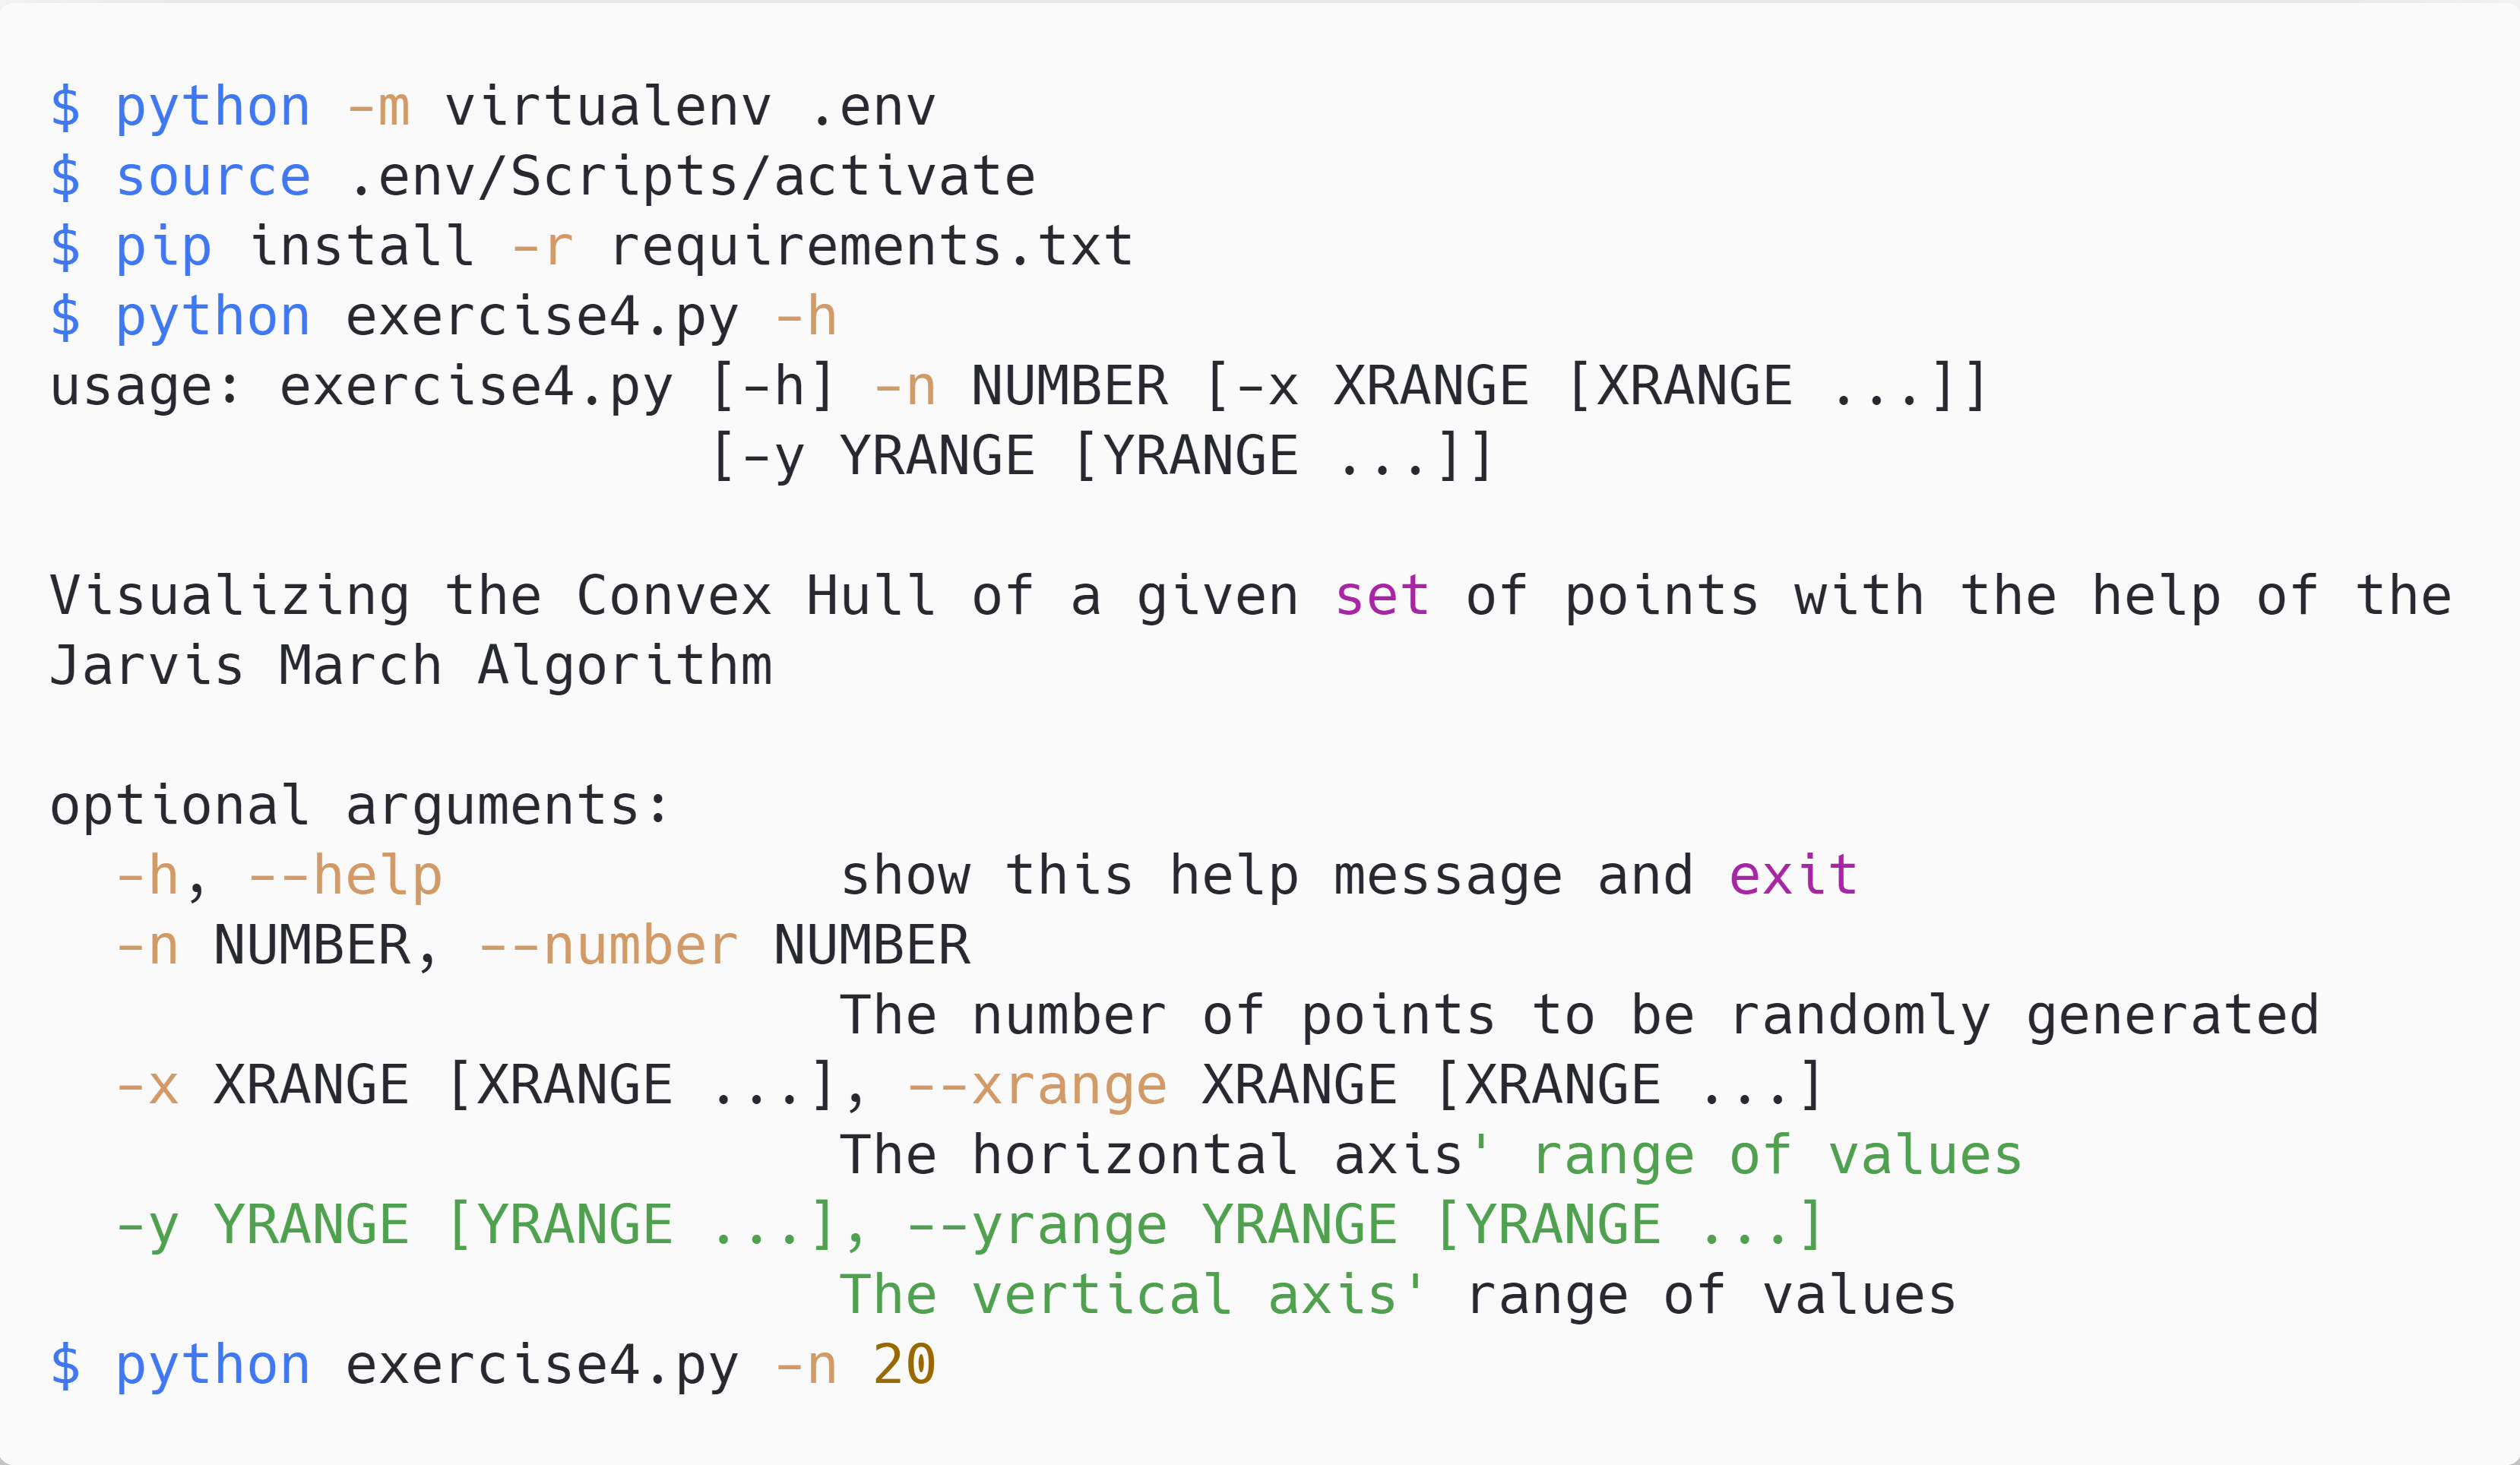
\includegraphics[scale=0.140]{images/gift_wrapping_algorithm.png}
    \caption{Οδηγίες εκτέλεσης προγράμματος}
\end{matlab}

\subsubsection*{Example Usage}

\begin{matlab}
    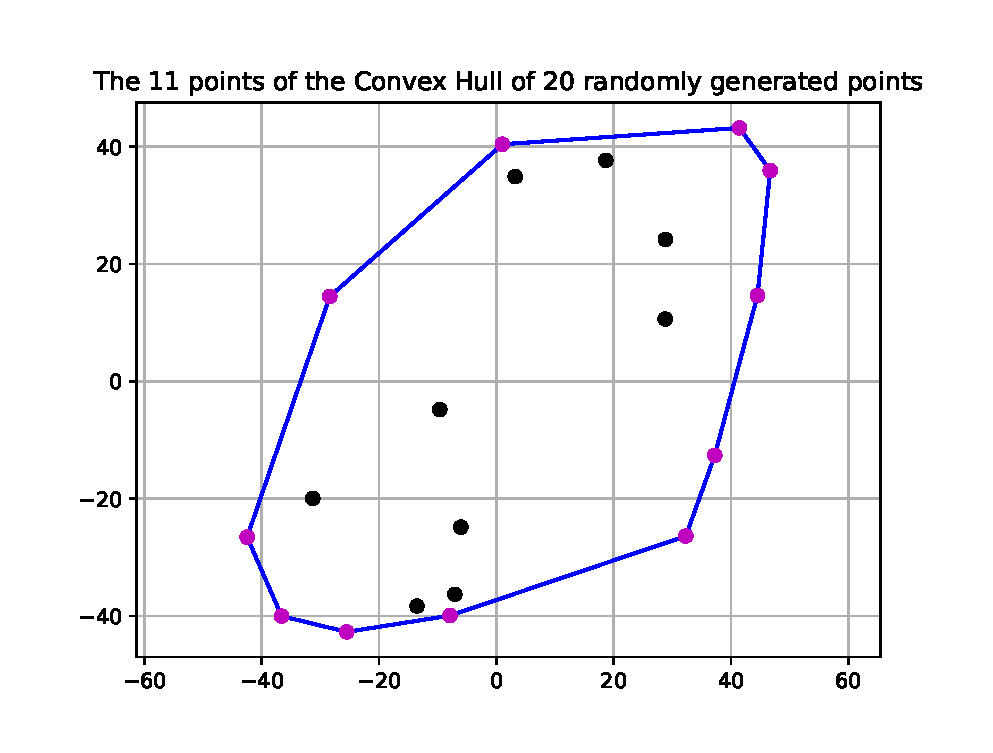
\includegraphics[scale=1]{images/gift_wrapping_algorithm.eps}
    \caption{Ενδεικτική έξοδος του προγράμματος}
\end{matlab}

\pagebreak

\end{document}
